\section{Durchführung}
\label{sec:Durchführung}
\subsection{Einseitige Einspannung}
\label{sec:eins}
\begin{figure}
  \centering
  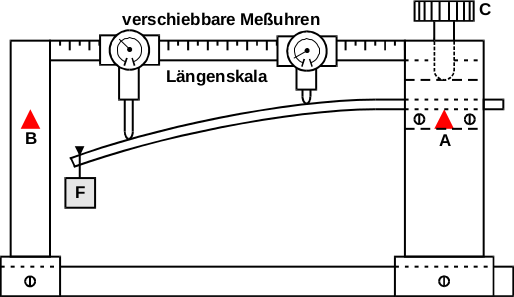
\includegraphics[width=0.8\textwidth]{content/images/Abbildung2.png}
  \caption{Versuchsaufbau bei der einseitigen Einspannung.}
  \label{fig:abb2}
\end{figure}
Bei der einseitigen Einspannung werden zwei verschiedene Metallstäbe ausgemessen
und gewogen, und anschließend unter einer Messuhr, gemäß \ref{fig:abb2}, eingespannt.
Aus Gewicht und Abmessungen wird die Dichte des Metalls, und anhand von Literaturwerten
\cite{litval} das Metall an sich, bestimmt. Ist das Metall eingespannt wird zunächst
die Länge des frei hängenden Stabes, sowie die Masse des Gewichtes, gemessen. Hiernach geschieht die eigentliche Messung,
bei welcher alle \SI{2}{\centi\meter} die Auslenkung $D(x)$ je mit und ohne Gewicht gemessen wird.
Durch die Differenz dieser beiden Werte ergibt sich die zur Auswertung benötigte Auslenkung. Dies wird für den
2. Stab wiederholt.
\subsection{Beidseitige Einspannung}
\label{sec:beid}
Bei der beidseitig einespannten Messung wird einer der Stäbe aus \ref{sec:eins}
verwendet und die eingespannte Länge durch die Gesamtlänge der Messapperatur bestimmt.
Daher bleibt zur vorbereitenden Messung lediglich die neue Masse des Gewichtes, welches hier
in der Mitte des Stabes angebracht ist, zu bestimmen. Die eigentliche Messung wird erneut durch
die Notation der Differenz der Auslenkungen mit und ohne Gewicht alle \SI{2}{\centi\meter} durchgeführt.
